% This is LLNCSDOC.TEX, the documentation file of
% the LaTeX2e class from Springer-Verlag
% for Lecture Notes in Computer Science, version 2.24
\documentclass[runningheads]{llncs}
% Add PDF bookmarks and metadata
\usepackage[bookmarksopen,
bookmarksopenlevel=1,
bookmarksdepth=2,
pdftex,
pdfauthor={No Author Given},
pdftitle={Instantaneous, Understandable, and Actionable Soundness Checking of Industrial BPMN Models},
pdfsubject={BPMN soundness checking},
pdfkeywords={BPM, BPMN, BPMN analysis, Soundness checking}
]{hyperref}
%
\usepackage{graphicx}
% If you use the hyperref package, please uncomment the following line
% to display URLs in blue roman font according to Springer's eBook style:
% \renewcommand\UrlFont{\color{blue}\rmfamily}

\begin{document}
%
\title{Instantaneous, Understandable, and Actionable Soundness Checking of Realistic BPMN Models}
%
\titlerunning{Instantaneous Soundness Checking of Industrial BPMN Models}
% If the paper title is too long for the running head, you can set
% an abbreviated paper title here
%
% \author{Tim Kr\"{a}uter\inst{1}\orcidID{0000-0003-1795-0611} \and
% Adrian Rutle\inst{1}\orcidID{0000-0002-4158-1644} \and
% Harald K\"{o}nig\inst{2,1}\orcidID{0000-0001-6304-6311} \and
% Yngve Lamo\inst{1}\orcidID{0000-0001-9196-1779}}
% \authorrunning{T. Kräuter et al.}
% \institute{Western Norway University of Applied Sciences, Bergen, Norway
% \email{tkra@hvl.no, aru@hvl.no, yla@hvl.no} \and
% University of Applied Sciences, FHDW, Hanover, Germany\\
% \email{harald.koenig@fhdw.de}}
%
\maketitle              % typeset the header of the contribution
%
\begin{abstract}
TODO
\keywords{
Business Process Modeling \and
Verification \and
BPMN Soundness\and
Quality assurance
}
\end{abstract}

% Up to 16 pages, including everything!

% Redefine enumerations
\renewcommand{\labelenumi}{(\textbf{\arabic{enumi})}}

\section{Introduction} \label{sec:introduction}

% Problem statement
% Why useful?
\cite{fahlandAnalysisDemandInstantaneous2011}
% Claims a lot of problems in workflow models, which can be found using soundness checks.

% Motivation

% Solution
% Describe the figure and go over all three claims briefly: instantaneous (Definition), understandable (soundness properties are hard to understand for modelers), and actionable (comparable to quick fixes).

% Also add the times measured by other tools for some models. These range into seconds? Would be nice to try the sasme models later.

% Understandable/Visualization is missing in the figure: instantaneous and actionable are there.
\begin{figure}[ht]
	\centering
	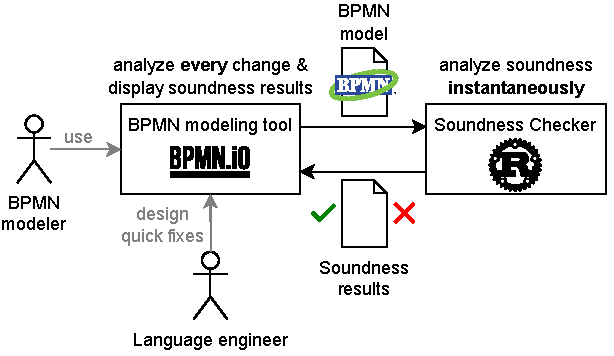
\includegraphics[width=0.7\textwidth]{images/overview}
	\caption{Overview of the approach}
	\label{fig:overview}
\end{figure}

% What do the results contain? If wrong: Counterexample and problematic elements

% Soundness stuff taken from which adopted it for BPMN
\cite{corradiniClassificationBPMNCollaborations2018}

% One example should be introduced here, which then is picked up throughout the paper.
% Wrong gateway usage?
% Instantaneous: The model checks in 500ms or less.
% Understandable: Highlight problematic elements + show the visualization of a counterexample using that model.
% Actionable: Provide quick fixes that resolve soundness violation --> check if changes fix the property before showing it to the user.

\section{Soundness Checking of BPMN Models}

% Describe soundness checking for BPMN models.
Soundness was introduced for workflow nets in \cite{vanderaalstAPPLICATIONPETRINETS1998} and stems from the field of Petri Nets.
We will use the formal definition directly given for BPMN by \cite{corradiniClassificationBPMNCollaborations2018}.

% Soundness actually does not include safeness.
Soundness is composed of three following sub-properties \cite{corradiniClassificationBPMNCollaborations2018}:
\textit{(i) Option to complete}: any running process instance must eventually complete,
\textit{(ii) Proper Completion}: at the moment of completion, each token of the process instance must be in a different end event, and
\textit{(iii) No dead activities}: any activity can be executed in at least one process instance.

In addition, we also check \textit{safeness}.
A BPMN model is \textit{safe} if during its execution no more than one token occurs along the same sequence flow \cite{corradiniClassificationBPMNCollaborations2018}.


\section{Instantaneous Soundness Checking} \label{sec:instantaneous}
\textit{Instantaneous} soundness checking is defined as taking 500 ms or less in~\cite{fahlandAnalysisDemandInstantaneous2011}.
In this section, we demonstrate that our soundness checker is instantaneous by validating it from three different viewpoints.
First, we investigate how our tools reacts to rapidly \textit{growing model size} in \autoref{subsec:model-size}.
We use a benchmark based on synthetically generated BPMN models.
% also called levels of concurrency in fahlandAnalysisDemandInstantaneous2011 ? degrees of paralleism somewhere else by the italians.
Second, we study how our tool deals with \textit{growing degrees of parallelism} in \autoref{subsec:degrees-of-parallelism}
Third, we input industrial models identified in other publications or coming from public data sets into our tool and measure the performance.
Third, we run soundness checking for several industrial BPMN process models identified in other studies or available in public datasets, see \autoref{subsec:industrial-models}. % Add some citations here or later once we did this.
%These guys have some benchmarks:
%\cite{corradiniFormalApproachAnalysis2021}

% General info
% We use hyperfine for each benchmark with runs stuff 10x and averages? See my other papers
For all our benchmarks, we use the hyperfine benchmarking tool~\cite{peterHyperfine2023} (version 1.18.0), which calculates the average runtime when executing each soundness check ten times.
The benchmarks were run on a Windows 11 machine with an AMD Ryzen 7700X processor and 32 GB of RAM~\cite{noauthorgivenBPM2024Artifacts2024}.

% Artifacts using a Zenodo link at the end. Maybe my anonymous github account before.
All used BPMN models are given in the artifacts of this paper~\cite{noauthorgivenBPM2024Artifacts2024}.
Furthermore, we provide the scripts to replicate our benchmarks using hyperfine.

% Improve this and explain the reasoning is inspired by corradiniFormalApproachAnalysis2021

\subsection{Growing Model Size} \label{subsec:model-size}
We use the data-set of models provided in~\cite{krauterHigherorderTransformationApproach2023}, which consists of 300 synthetically generated BPMN models.
% Briefly recap the method.
Every BPMN model contains a start event, a fixed amount of \textit{blocks}, and an end event.
The number of blocks ranges from 1 to 300 and there are three different blocks that are used repeatedly.
\autoref{fig:three-block-example} shows the third BPMN model in the data-set which contains each of the different blocks once.

\begin{figure}[ht]
	\centering
	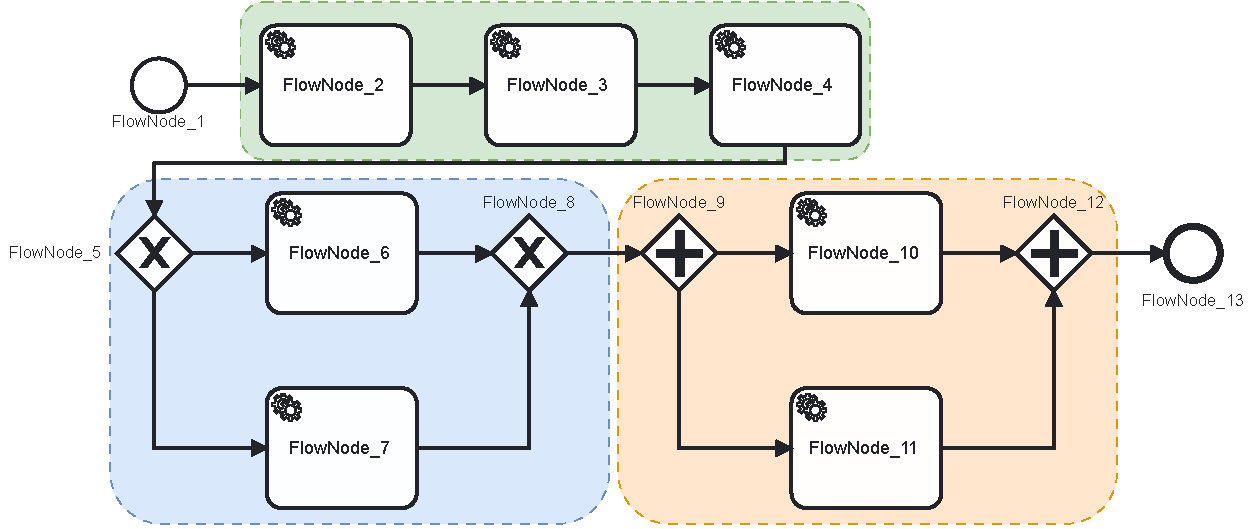
\includegraphics[width=0.9\textwidth]{images/three-blocks}
	\caption{BPMN model with three blocks~\cite{krauterHigherorderTransformationApproach2023}}
	\label{fig:three-block-example}
\end{figure}

\autoref{fig:model-size-benchmark} shows the average runtime of our tool when checking soundness for the BPMN models with increasing model size.
Each model is sound which means that our tool exhaustively searches the state space.

\begin{figure}[ht]
	\centering
	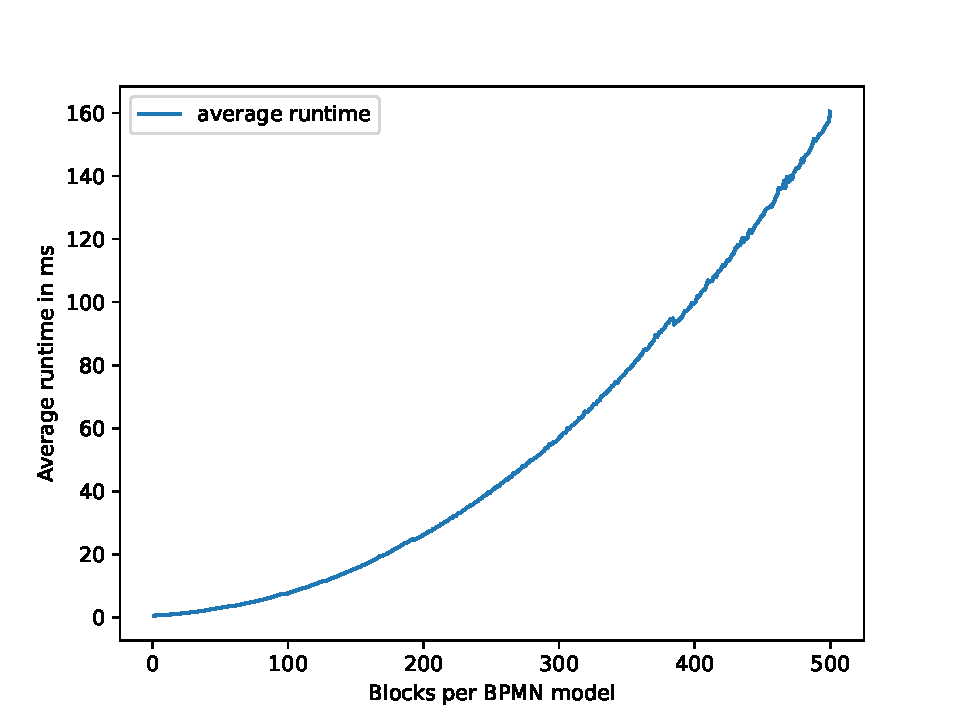
\includegraphics[width=0.7\textwidth]{images/model-size-benchmark}
	\caption{Soundness checking runtime for models of increasing size}
	\label{fig:model-size-benchmark}
\end{figure}

% Results
Once can see that our tools spends starting from 10 ms up to 100 ms for the BPMN models.
Thus, our tool can check soundness instantaneously according to our definition in \autoref{sec:introduction} even if model size increases to over 2400 BPMN elements as in the synthetic data-set provided in~\cite{krauterHigherorderTransformationApproach2023}.
Models of this size are not human readable anymore and are divided into smaller models according to best-practices \cite{fahlandAnalysisDemandInstantaneous2011}.
Thus, models found in practice are likely to be smaller than in our benchmark and we can check large number of models in parallel if needed.

\subsection{Growing Number of Parallel Branches} \label{subsec:degrees-of-parallelism}
% Cite the other paper here with parallelism and introduce the set of models.
An increase in model size leads to a bigger state space of the model that must be analyzed for soundness and safety.
% States for the previous:
% 1: 5 states, 5 transitions
% 50: 218, 218
% 100: 434, 434
% 150: 652, 652
% 200: 868, 868
% 250: 1084, 1084
% 300: 1302, 1302
In the previous section a linear increase in model size lead to a similar growth in the state space.
However, models with a growing number of parallel branches lead to an exponential increase in the state space, i.e., a state space explosion.
In this section, we test our tool against a synthetic data set of models which lead to state space explosion.

We generate a data set of models with a growing number of parallel branches, similar to the ones described in \cite{corradiniFormalApproachAnalysis2021}.
\autoref{fig:parallel-branches-models} depicts how a model with \textit{n} parallel branches is generated.

\begin{figure}[ht]
	\centering
	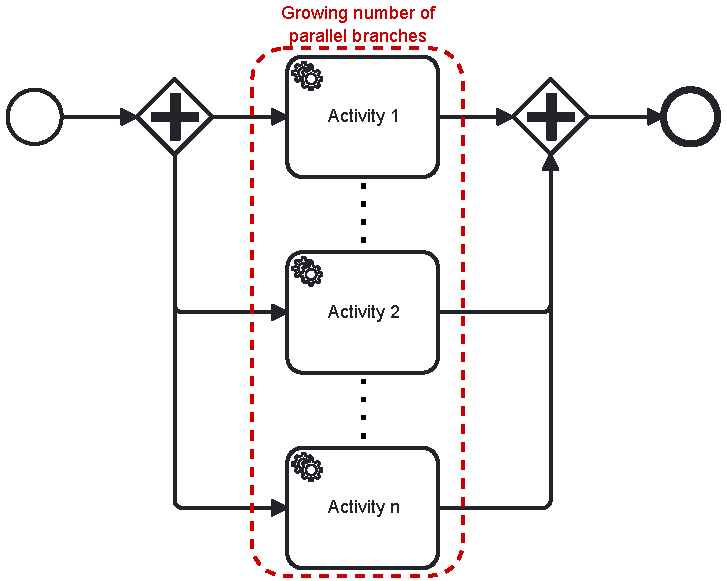
\includegraphics[width=0.5\textwidth]{images/growing-number-of-parallel-branches}
	\caption{Models with a growing number of parallel branches (similar to \cite{corradiniFormalApproachAnalysis2021})}
	\label{fig:parallel-branches-models}
\end{figure}


\autoref{fig:parallel-branches-benchmark} shows the average runtime of our tool when checking soundness for the BPMN models with increasing degree of parallelism.
Each model is sound which means that our tool exhaustively searches the state space.

% Do a benchmark from p01-p20 or higher? --> Memory issues.
% Maybe a table is even better than a plot here. if its "just" 20 lines we can display more information like state space etc.
% Exponential state space growth (2^x + 3, start, pre end, and end state)
\begin{figure}[ht]
	\centering
	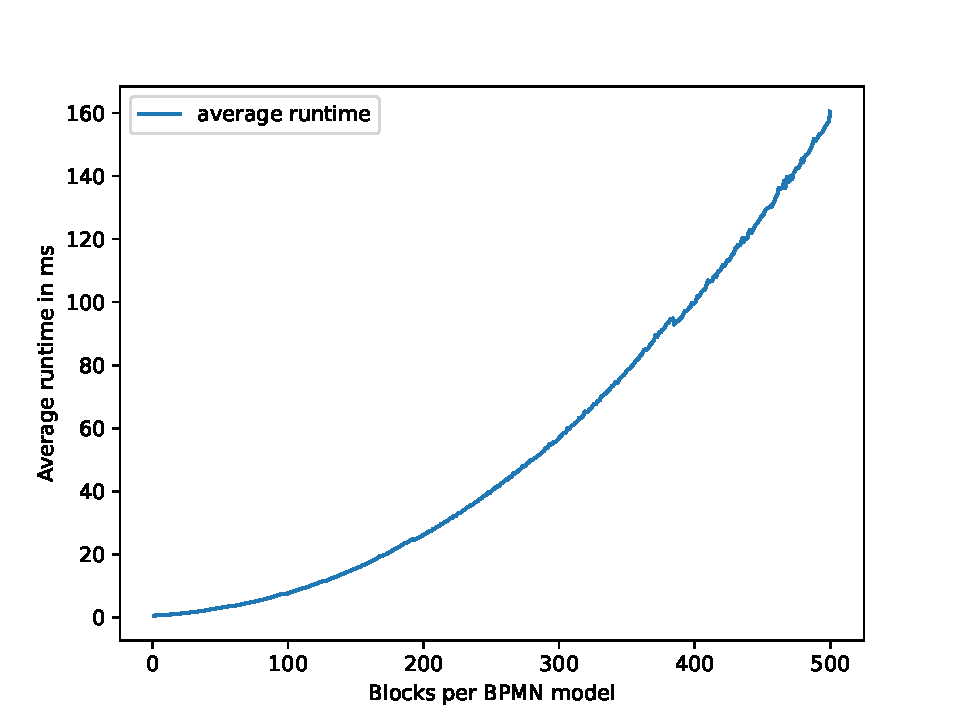
\includegraphics[width=0.7\textwidth]{images/model-size-benchmark}
	\caption{Soundness checking runtime for models with increasing parallel branches}
	\label{fig:parallel-branches-benchmark}
\end{figure}

The state space of the models grows exponentially (in our case $2^x$) when increasing the degree of parallelism which shows that BPMN models can exhibit the state space explosion problem. % Cite something here?
Thus, our analysis stops being reasonable after x and being instantaneous after y.
We will discuss later if models with such a high degree of parallelism are realistic.

\subsection{Realistic Models} \label{subsec:industrial-models}
% Maybe rename to real world and use the models in corradiniFormalApproachAnalysis2021.

% Check that we can analyze models from the model repositories cited anywhere.
% Especially look for models to be "industrial"! --> some in my previous publications were.
% Pick 5-10 models and add a table or a summary and a table in the artifacts?

\subsection{Discussion}
% Summarize and discuss further points
% The implementation is in the sense unoptimized but already works great for the models we have tested.
% Partial-order reduction especially and other optimization techniques might be applied in the future if the needs arise.
% escpecially fahlandAnalysisDemandInstantaneous2011 advocates for partial order reduction. It solves exactly this problem.
% But do we really get such models in practice? We would say no but if we do we need partial order reduction techniques which show great promise in fahlandAnalysisDemandInstantaneous2011 and make models with greater state spaces tractable.
% For proper completion, dead activities, option to complete the order in which the parallel branches execute probably does not matter.
% Safeness could be more difficult. But one can probably reuse/adapt what has been done in the petri nets domain. If this really is a problem.

% Also check memory usage.

\section{Understandable Soundness Checking}

The first step to fixing a soundness violation is understanding the problem.
Thus, a tool must present soundness violations clearly with the necessary details to the BPMN modeler.
We aim to make soundness checking understandable by not only providing textual feedback but rather utilizing the graphical structure of the BPMN model.

% Identify problematic elements using overlays.
We highlight the problematic elements in the BPMN model, which cause soundness violations.
\autoref{fig:violations} depicts how we highlight problematic elements using red overlays in our tool.
In addition, there is a summary panel in the top-right corner.

\begin{figure}[ht]
	\centering
	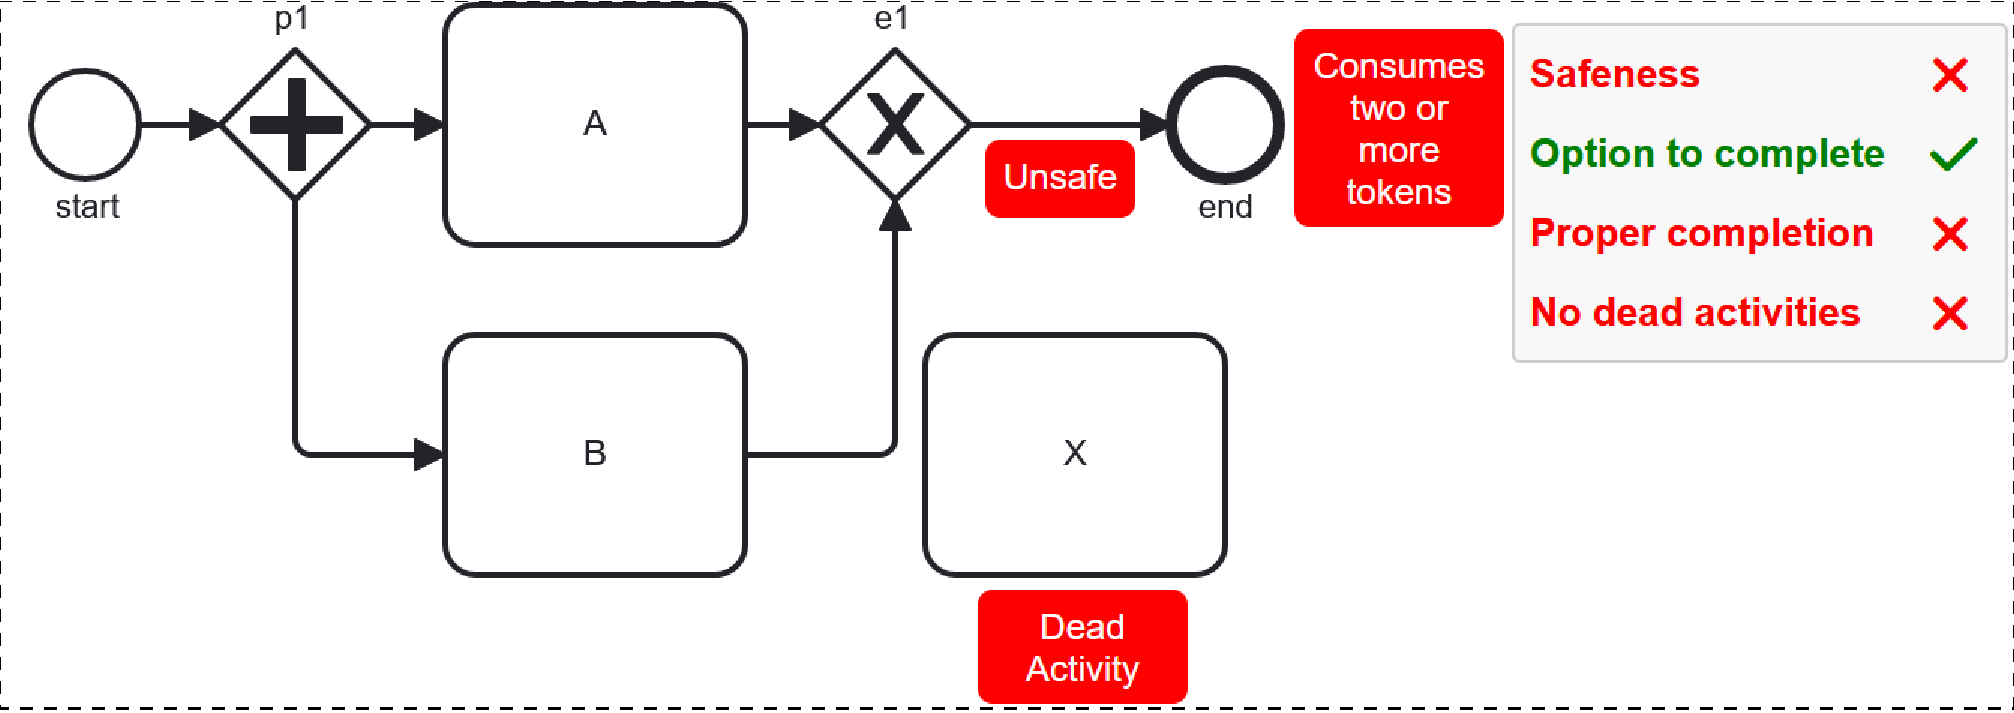
\includegraphics[width=0.9\textwidth]{images/violations}
	\caption{\textit{Soundness violations} in the analysis tool}
	\label{fig:violations}
\end{figure}

Using the overlays one can immediately see which elements cause soundness violations which helps to pinpoint the root problems in the BPMN models.
For \textit{safeness} we highlight sequence flows that can become \textit{unsafe}, i.e., two tokens can be located at the sequence flow.
For \textit{proper completion} we identify the end events that can consume more than one token, while for \textit{no dead activities} we highlight the dead activities in the BPMN model.
For \textit{option to complete} we cannot highlight elements since it means the process execution can get stuck which cannot easily be attributed to single BPMN elements.
% --> Seen partly in other tools

% Interactive visualization of counterexamples. --> Not seen before. some allow exports of counter examples but no direct interaction --> reduction of friction.
However, just by looking at the BPMN model it can still be hard to understand soundness violations due to the interplay of the BPMN elements execution semantics.
In the BPMN specification, execution semantics are described using the concept of moving \textit{tokens}~\cite{objectmanagementgroupBusinessProcessModel2013}.
% Universally used concept of tokens
The concepts of tokens is used in BPMN tools in the industry to depict process execution information~\cite{camundaservicesgmbhBpmnjsTokenSimulation2024} and in many BPMN formalizations~\cite{vangorpVisualTokenbasedFormalization2013,krauterFormalizationAnalysisBPMN2023,houhouFirstOrderLogicVerification2022,corradiniFormalisingAnimatingMultiple2022}.

We use tokens in our tool to \textit{interactively} visualize the counter examples, i.e, violation witnesses of our soundness properties.
Our soundness checker provides counter examples for all properties besides no dead activities.
Then we visualize these counter examples directly in the BPMN editor by showing how tokens move from the process start to a state which violates the given soundness property.
\autoref{fig:counter-example} shows a screenshot visualizing the safeness counter example for the same BPMN model as shown in \autoref{fig:violations}.

% A bit wasteful regarding space due to the execution log.
\begin{figure}[ht]
	\centering
	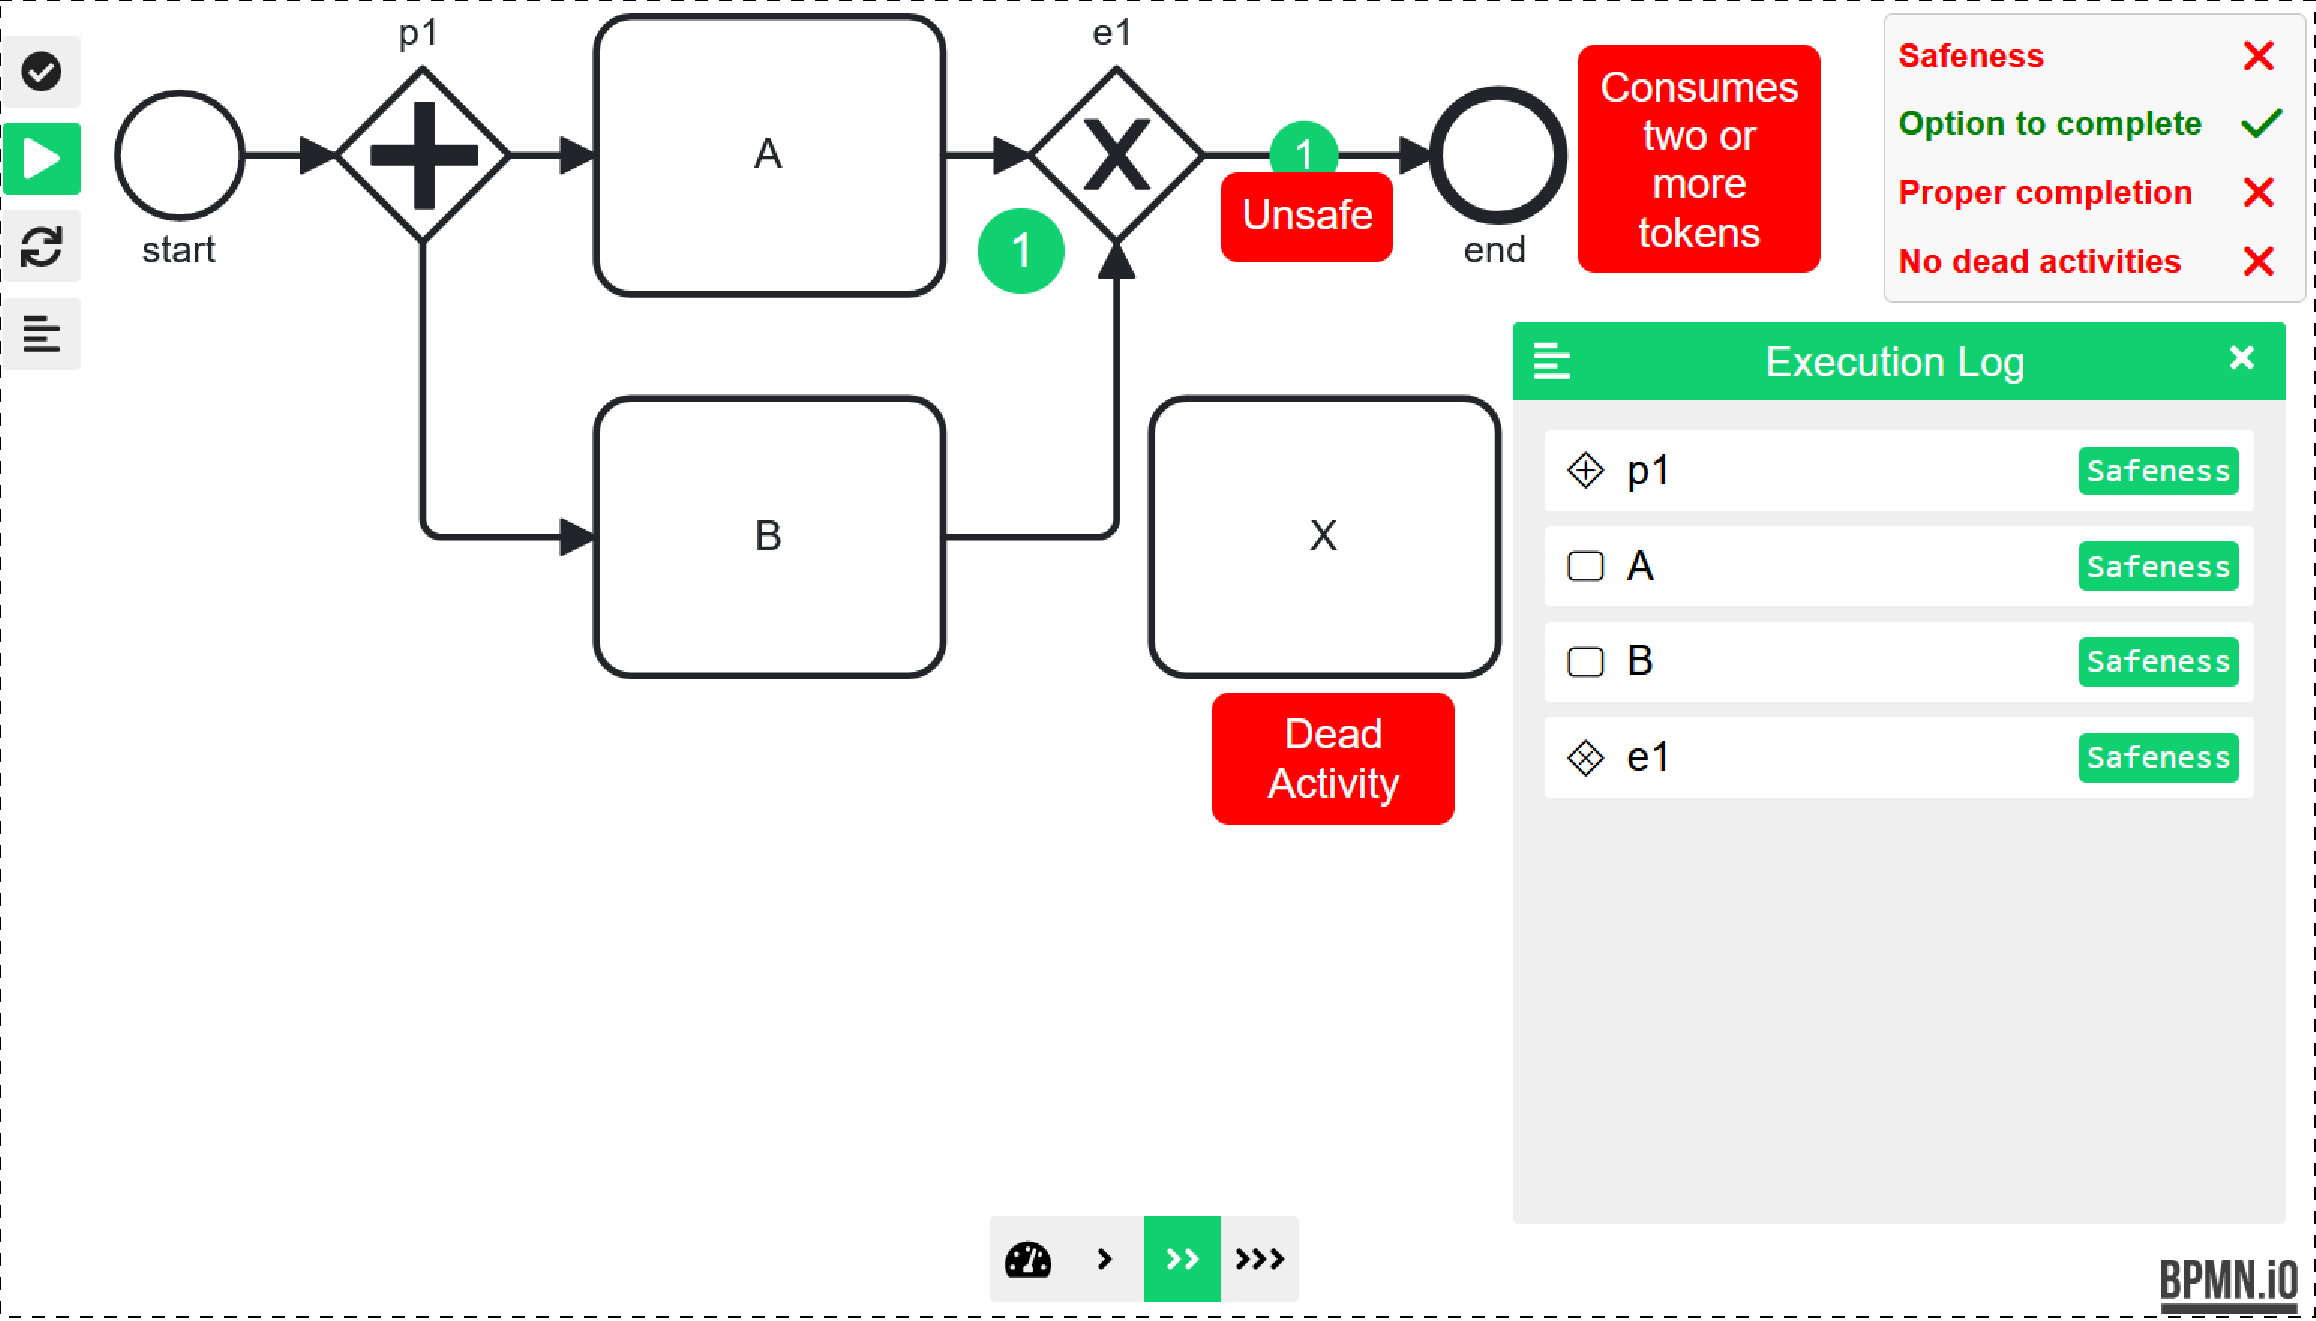
\includegraphics[width=0.9\textwidth]{images/counter-example}
	\caption{Interactive \textit{counter example visualization} in the analysis tool}
	\label{fig:counter-example}
\end{figure}

% Describe the figure.
In \autoref{fig:counter-example} the visualization has been \textit{paused} just before the \textit{unsafe} state was reached.
One token is already located at the sequence flow which is marked as unsafe while a second token is currently waiting at the exclusive gateway \textsf{e1}.
The visualization can be resumed or restarted using the play and restart button on the left side.
When resumed, the gateway \textsf{e1} will execute, resulting in two tokens located at the subsequent sequence flow, i.e., an unsafe execution state.
In addition, one can control the visualization speed using the bottom buttons next to the speedometer.

% Execution log
Furthermore, our tool shows an \textit{execution log} which states the history in which BPMN elements have been executed.
In \autoref{fig:counter-example} the parallel gateway \textsf{p1}, the activities \textsf{A} and \textsf{B}, as well as the exclusive gateway \textsf{e1} have each been executed once before the pause.
This is useful since often an unsuspected execution order leads to property violations.

% Conclusion for understandable
In summary, we aim to make soundness checking easily \textit{understandable} even for users unaccustomed to the BPMN execution semantics.
First, we directly highlight problematic elements in the BPMN editor.
Second, we provide an \textit{interactive} visualization of counter examples in the BPMN editor with the ability to pause the visualization, control the visualization speed, and show an execution log which makes understanding the property violation straightforward.

\section{Actionable Soundness Checking}

When possible, we detect errors in the BPMN model and provide an automatic fix similar to \textit{quick fixes} in Integrated Development Environments (IDEs).
Modelers can then select these quick fixes to resolve a soundness property violation.
\autoref{fig:quick-fixes} shows a screenshot of our tool, where quick fixes are depicted as green overlays containing a light bulb icon.
This icon is typically used to indicate quick fixes in IDEs.
Our tool simultaneously shows soundness violations (\autoref{fig:violations}) and quick fixes (\autoref{fig:quick-fixes}).

\begin{figure}[ht]
	\centering
	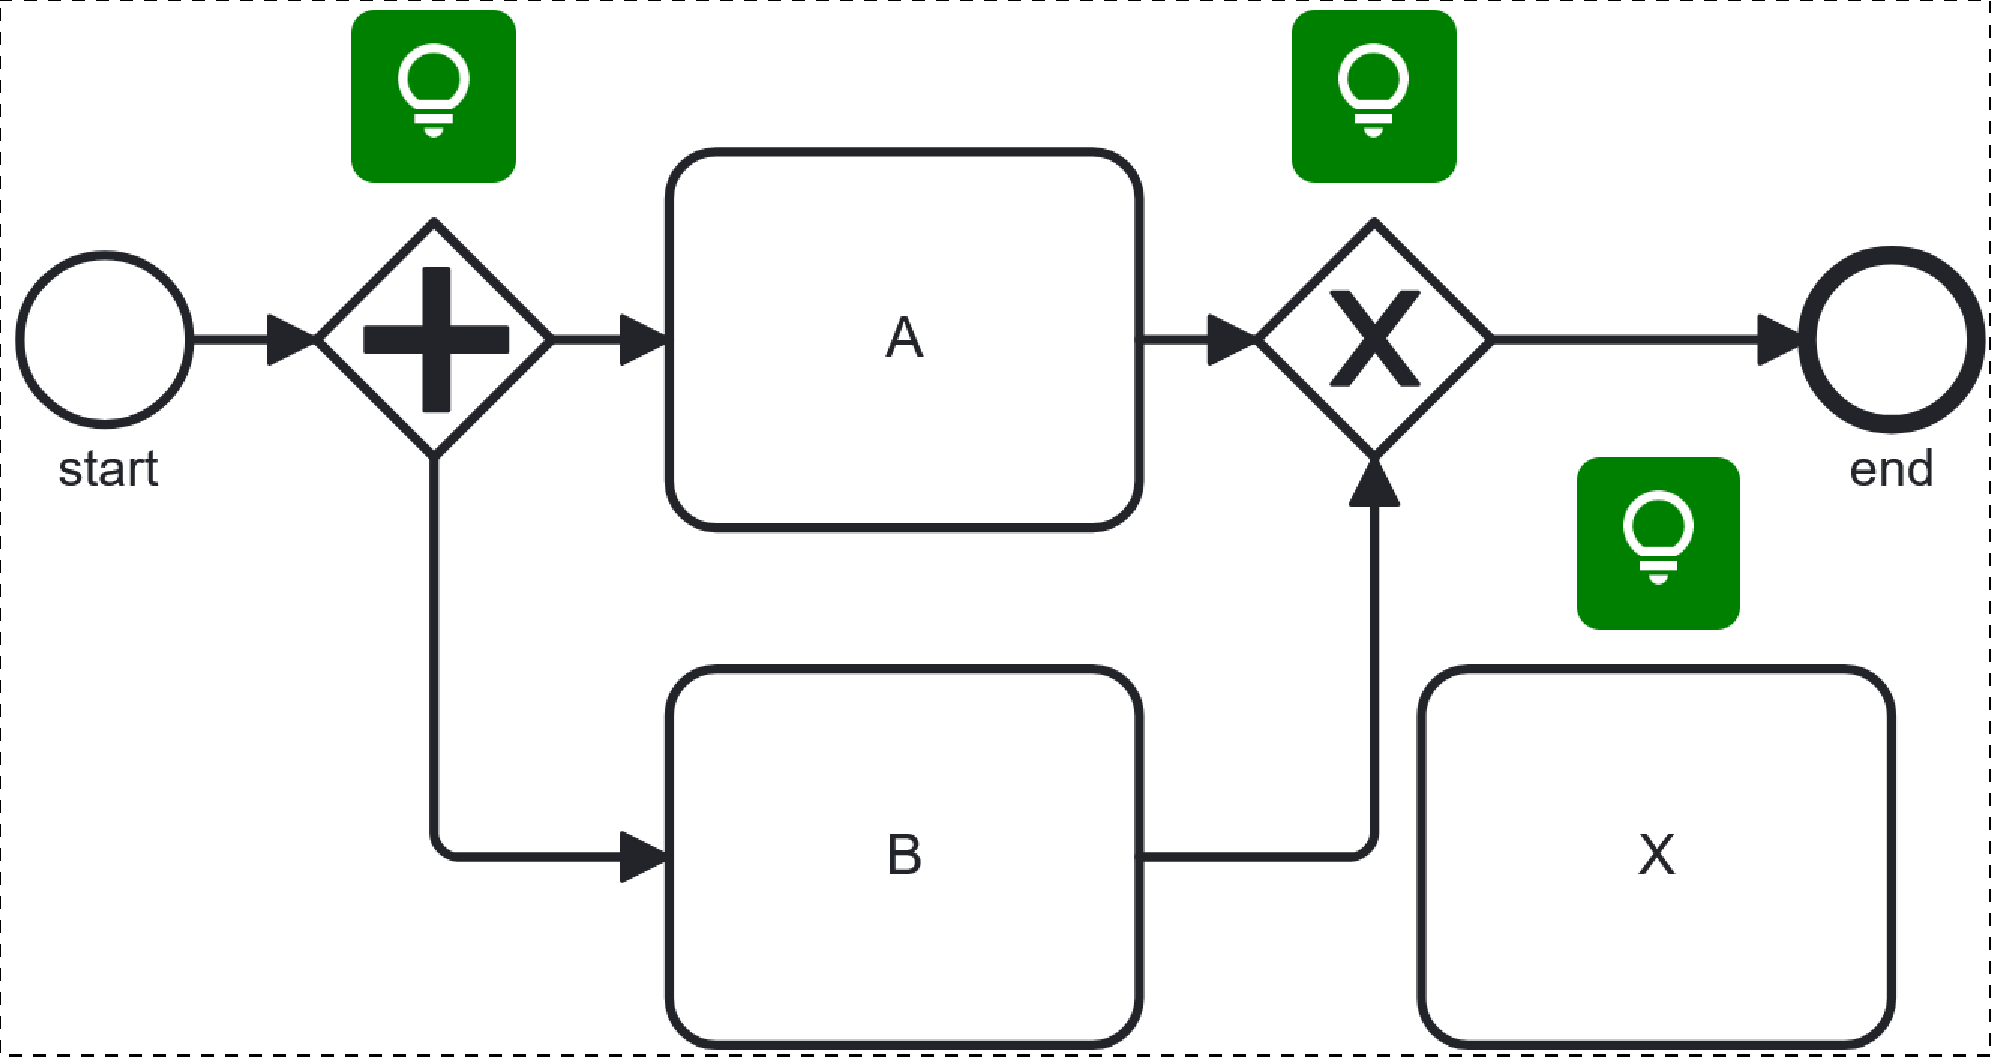
\includegraphics[width=0.6\textwidth]{images/quickfixes}
	\caption{\textit{Quick fixes} in the analysis tool}
	\label{fig:quick-fixes}
\end{figure}

The user can apply a quick fix by clicking on the green overlays and immediately see the changes in soundness since checking is \textit{instantaneous} as discussed in \autoref{sec:instantaneous}.
If he is unhappy with the result, a user can undo these changes immediately since each quick fix is a \textit{command} (see command pattern~\cite{gammaDesignPatternsElements1995}).
A user might not like a quick fix if it not only fixes a specific property but also has unintended side effects.
For example, it might invalidate a different soundness property.

In the following sections, we describe the implemented resolution strategies for the different soundness properties in detail.
However, we do not expect these strategies to cover all possible resolutions and fit all applications.
Thus, our framework is extensible, so other developers can provide additional or custom resolution strategies.
This is possible since we \textit{decoupled} the soundness analysis from showing violations and providing quick fixes in our implementation, which facilitates customization by using dependency injection.

\subsection{Safeness} \label{subsec:safeness}
The soundness checker will provide a counter-example and identify the unsafe sequence flows.
We use this information together with the structure of the BPMN model to find resolutions for \textit{Safeness} violations.
In general, safeness violations can have multiple reasons.

\begin{enumerate}
	\item An exclusive gateway with multiple incoming sequence flows activated more than once will lead to multiple tokens at its outgoing sequence flows.
	\item One can also implicitly encode an exclusive gateway, for example, using an activity, by having multiple incoming sequence flows.
	Implicitly encoding exclusive gateways is allowed but violates best practices (see lint rule \textit{fake-join} in~\cite{camundaservicesgmbhBpmnlint2024}).
	Similar to \textbf{(1)}, this leads to unsafe sequence flows if activated more than once.
\end{enumerate}


\textbf{Resolutions for (1):} A straightforward solution is to change the exclusive gateway to a parallel one.
Since the gateway was activated multiple times it indicates that it perhaps should have been a parallel gateway or there was an unintended parallelization before.
Thus, we can analyze the BPMN model and find the parallelization that causes the \textit{Safeness} violation.
If it is a parallel gateway, another solution is to change this parallel gateway to an exclusive one.
So, there are two solutions, but the goal is to have matching gateways.
The parallelization can also be an implicitly encoded parallel gateway, for example, an activity with multiple outgoing sequence flows, which does not comply with best practices but is allowed.
In this case, we can add an exclusive gateway to eliminate the implicit parallelization and achieve matching gateways.
% It would be nice to mention the command here already.

\textbf{Resolutions for (2):} Similarly to \textbf{(1)}, the goal of each quick fix is to obtain matching gateways.
Thus, one solution is to find the parallelization that causes the \textit{Safeness} violation and change it to an exclusive gateway, as described in \textbf{(1)}.
Quick fix \textbf{(a)} in \autoref{fig:safeness} shows this solution, where a parallel gateway is changed to an exclusive one.
We color all changes and additions green in figures, highlighting quick fixes.
Another solution is to remove the implicit exclusive gateway and add a parallel gateway instead, see quick fix \textbf{(b)} in \autoref{fig:safeness}.
The quick fix moves elements automatically to make space to insert the parallel gateway and then reconnects as well as adds sequence flows accordingly.
Even though these are multiple individual operations, we ensured that an undo operation would revert the whole quick fix.
All the implemented quick fixes can be reverted using one simple undo operation.

\begin{figure}[ht]
	\centering
	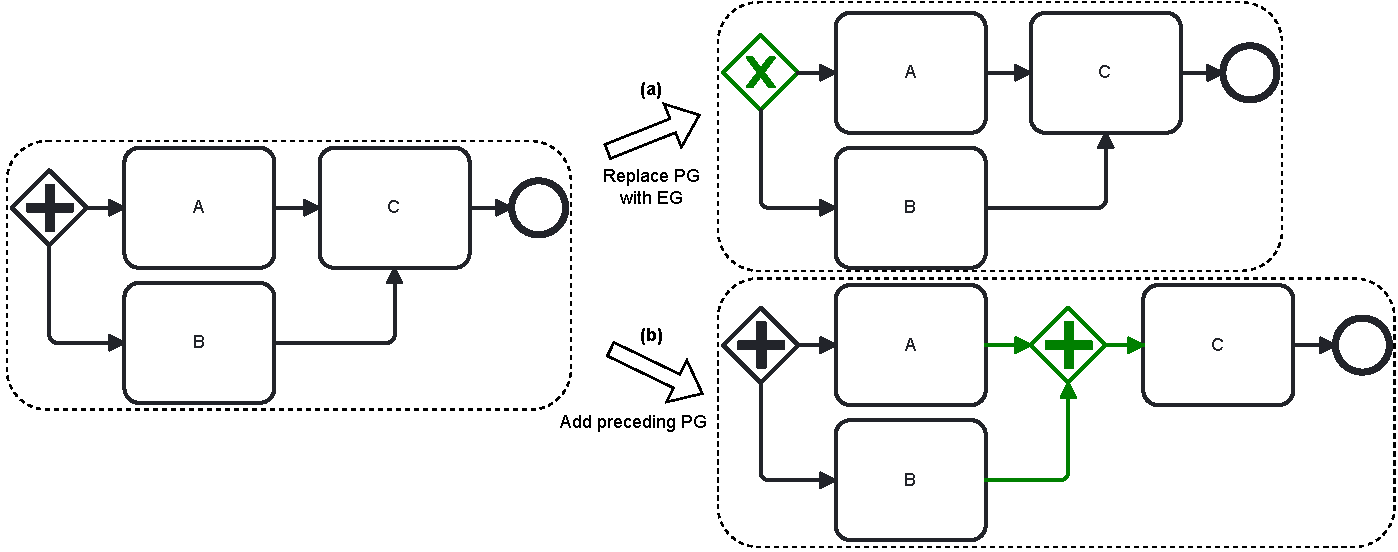
\includegraphics[width=1\textwidth]{images/safeness}
	\caption{Example quick fixes for \textit{Safeness}}
	\label{fig:safeness}
\end{figure}

% TODO: Add demo application and artifacts anonymously.
Our demo application in x contains examples of the Safeness quick fixes and all other soundness properties.

\subsection{Proper Completion}
The soundness checker will provide a counter-example and the end events that consume more than one token.
Violations of \textit{Proper Completion} at a specific end event can have multiple reasons.

\begin{enumerate}
	\item An end event can have multiple incoming sequence flows that can hold tokens.
	This could be due to a parallelization that is never synchronized.
	\item If there is only one incoming sequence flow, then this flow must be unsafe, i.e., hold more than one token in a possible execution.
\end{enumerate}

\textbf{Resolution for (1):} If multiple incoming sequence flows are the cause, we can add a unique end event for each except the first.
\autoref{fig:properCompletion} shows an example of this quick fix being applied, where the changed elements are colored in green.
We ensured that an undo operation would revert the quick fix using the command pattern~\cite{gammaDesignPatternsElements1995}.

% Can save a lot of space in this figure if needed. Go to two activities and put them closer together
\begin{figure}[ht]
	\centering
	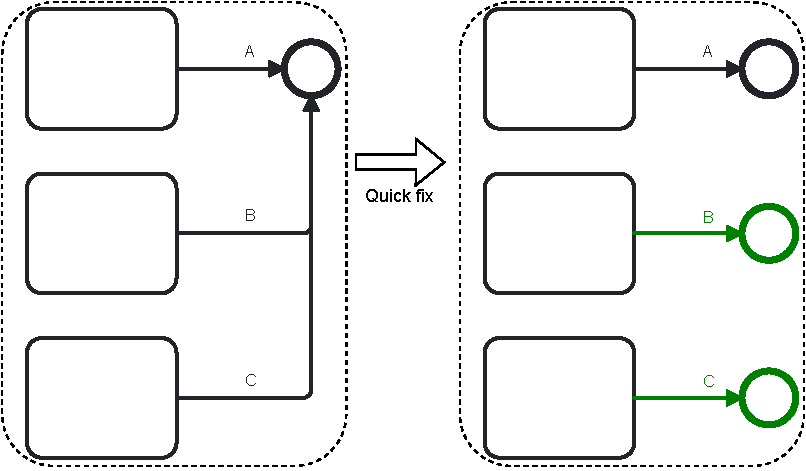
\includegraphics[width=0.7\textwidth]{images/properCompletion}
	\caption{Example quick fix for \textit{Proper Completion}}
	\label{fig:properCompletion}
\end{figure}

\textbf{Resolution for (2):} If a problematic end event only has one incoming sequence flow it must be unsafe.
Thus, other \textit{Safeness} quick fixes can apply, which will also resolve \textit{Proper Completion}, see \autoref{subsec:safeness}.


\subsection{Option to Complete} \label{subsec:optionToComplete}
Violations of \textit{Option to Complete} can have multiple reasons.

\begin{enumerate}
	\item A parallel gateway that synchronizes multiple incoming sequence flows but never executes leads to a violation.
	\item An event that is never triggered but relied upon in the process execution leads to a violation.
\end{enumerate}

To know the reason for a given violation, we analyze the counter example provided by the soundness checker.
The counter-example provides a trace that leads to a state in which the process cannot complete.
By analyzing the last state in this trace, i.e., the state in which execution cannot continue, we can determine which element is the cause.
Thus, we can provide quick fixes for the possible reasons.

\textbf{Resolutions for (1):} A straightforward way to fix sequence flow not continuing past a parallel gateway is to change it from parallel to exclusive.
Exclusive gateways do not synchronize, and thus, execution can continue.
\autoref{fig:optionToComplete} \textbf{(a)} shows an example of this quick fix where the replaced gateway is highlighted in green.

\begin{figure}[ht]
	\centering
	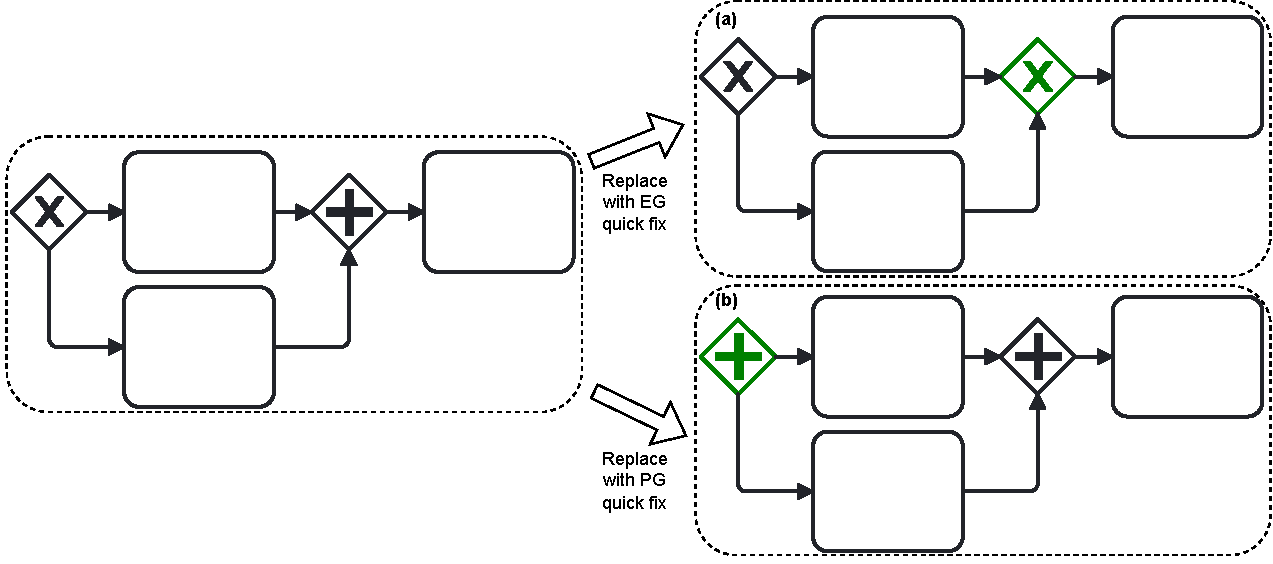
\includegraphics[width=1\textwidth]{images/optionToComplete}
	\caption{Example quick fixes for \textit{Option To Complete}}
	\label{fig:optionToComplete}
\end{figure}

Another way to fix violations is to find the split in the sequence flow, for example, the exclusive gateway in \autoref{fig:optionToComplete}, and make this split a parallelization, see quick fix \textbf{(b)} in \autoref{fig:noDeadActivitiesQuickFix}.
We present both possible resolutions to the user, who can choose the appropriate one.
Similar to the quick fixes

In the example in \autoref{fig:noDeadActivitiesQuickFix}, it is possible to spot the mismatching gateways.
However, this might not be straightforward in bigger BPMN models with more flow nodes and sequence flows.

\textbf{Resolutions for (2):} We have not yet implemented any quick fixes for events, but many interesting possibilities exist.
For example, for message catch events without incoming message flows, one could add a fitting message flow from a message throw event or send task.
One can use different factors, such as spatial proximity and name similarity, to find the right source of the new message flow.
The idea for any event would be to add the missing trigger.
Finding the most fitting trigger can be done in various ways by analyzing the other elements in the BPMN model.


\subsection{No Dead Activities}
A dead activity might have multiple reasons:

\textbf{(1):} The simplest reason is that the activity is disconnected, i.e., it has no incoming sequence flow.
Disconnected activities must not be dead, but they violate best practices see lint rule \textit{no-disconnected} in~\cite{camundaservicesgmbhBpmnlint2024}.

\textbf{(2):} An activity can also be part of the BPMN model that is not reachable during execution because a parallel gateway preceding the activity cannot be executed.
% Could also be behind events that are never triggered.

\textbf{Resolutions for (1)}: If the activity is disconnected, we can propose connecting it to the nearest flow-node.
However, this flow node should not be disconnected or dead itself.
Concretely, we assume modeling from left to the right, such as all the other automatic layout mechanisms in bpmn-js~\cite{camundaservicesgmbhBpmnjs2024} to find the leftmost nearest flow-node to connect.
\autoref{fig:noDeadActivitiesQuickFix} shows an example where this quick fix is applied.
As in the other examples, new elements are colored in green.

\begin{figure}[ht]
	\centering
	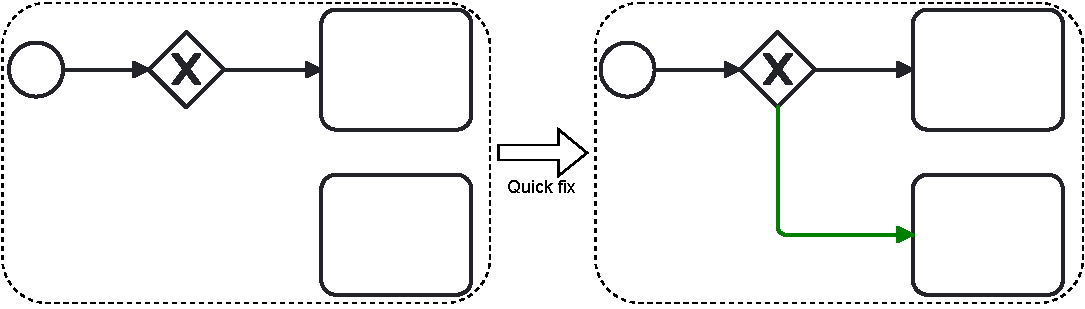
\includegraphics[width=0.6\textwidth]{images/dead}
	\caption{Example quick fix for \textit{No Dead Activities}}
	\label{fig:noDeadActivitiesQuickFix}
\end{figure}

\textbf{Resolutions for (2)}: When the dead activity is connected, this will often lead to processes that cannot terminate, i.e., violate \textit{Option to Complete}.
Thus, other quick fixes can apply, which will also resolve dead activities, see \autoref{subsec:optionToComplete}.

\section{Implementation}

% General goals: No friction for the modeler by integration into popular BPMN modeling tools.
% Modular structure such that it can be turned off our different features can be used or reused in different situations.
% We make use of the bpmn token simulation from camunda and generally the diagram-js/bpmn-js ecosystem.

\subsection{Rust}
% Why in Rust?
% Low-level language with modern features.
% Good for CLI tools such as this.
% Web assembly compilation? Client-side model checking in the browser? crazy talk

% Highlight Rusts speed and safety claims. Maybe cite some papers investigating this. Bottom line: Rust's performance is comparable to C and C++ with better development ergonomics and newer features (less cargo since it is a newer language).
% Zero-overhead abstractions --> related to speed
% Memory-management model in rust (Ownership, borrowing, and lifetimes) --> related to speed and performance
% Zero-copy? --> Currently, we are copying things but still achieve better performance (Tradeoff with readability)

% We chose rust mostly because of its performance regarding runtime and memory (no garbage collection).
% Memory is critical with increasing state spaces
% Speed is critical and should be linked to our motivation

\subsection{Pragmatic BPMN Semantics Encoding}
% Describe the runtime model. What is a state? --> Draw a UML diagram
% Describe what the initial state is. --> Could be configurable in the future.
% Describe BPMN semantics with some diagrams for some examples.
% Use a good running example with a modeling error that wasn't used before (double-blind).

Our minimal pragmatic BPMN semantics encoding that leads to comparably small state spaces and is sufficient to check soundness and safeness.
For example, \autoref{fig:activityEncoding} shows that we do not encode the start and end of a task but rather the execution as a whole.
This simple change avoids one additional state and pays off especially in models with many parallel branches, which can lead to significant reductions in the overall state space.

% Shows two encodings or state traces side by side. With ours having one less state
\begin{figure}[ht]
	\centering
	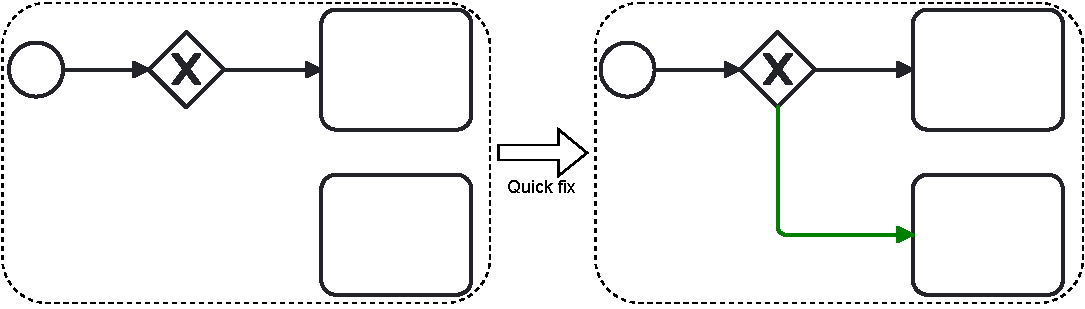
\includegraphics[width=0.6\textwidth]{images/dead}
	\caption{Minimal task execution encoding}
	\label{fig:activityEncoding}
\end{figure}

% For example: Message start events? Message events in general?
% Leaving tokens in front of gateways? Event-based gateway for example.
Similar, pragmatic encodings can be used for other BPMN elements to keep the state space as small as possible but still sufficiently detailed to check the given properties.
Nevertheless, one always must be sure that such simplifications do not compromise the properties that are checked, similar to partial-order reduction techniques.
In addition, the provided counter examples will be on the same level of detail as the BPMN encoding, which can make them simpler to follow or too simple to understand.
In summary, there is a trade-off between state space size which directly influences soundness checking runtime on the one hand versus implementation difficulty and understandability of counter examples on the other hand.

\subsection{Description}
% Tool UI with screenshot
\cite{camundaservicesgmbhBpmnjs2024}
% Tool architecture? UI in JS and backend in Rust. --> shown already earlier
% Just the model checker as a CLI app or a CLI that starts the whole thing as a service.

\section{Related Work}

% Different ways of comparison
% 1. BPMN features supported (sub of 2.)
% 2. Capabilities (Which soundness properties are supported, custom properties, counter-example visualization, tool maturity, tool integration, actionability of the tool, etc.) --> highlighting problematic elements is sometimes supported but interactive counter example visualization is not (to the best of our knowledge)
% 3. Performance using different benchmarks. --> Needs its own paper where everyone can contribute. --> Usually not done but quite important for industrial use. Model checking has to have adequate performance!
% We should mention the first two but focus on the third since this is where we shine. One and two can be improved in the feature if needed.

\cite{krauterFormalizationAnalysisBPMN2023,krauterHigherorderTransformationApproach2023}

\cite{vangorpVisualTokenbasedFormalization2013}

\cite{corradiniBProVeToolSupport2017,corradiniFormalApproachAnalysis2021}

\cite{houhouFirstOrderLogicSemantics2019,houhouFirstOrderLogicVerification2022}

Animation previously in \cite{corradiniFormalisingAnimatingMultiple2022,camundaservicesgmbhBpmnjsTokenSimulation2024} but not used for counter examples!


\section{Limitations \& Threats to Validity}

% Discuss linear model size increase i.e. no parallel degree increase --> BPMN models are linear in practice and much smaller than in this benchmark. cite instantaneous paper
% However, one could add more complex BPMN features than given in the three blocks shown there.

% Hard to really find industrial models?
% Other approaches are implemented in a more fomral setting and thus a comparison may not be apples to apples?
% We have build a specific tool for BPMN while other people have used generic tools: groove, maude, and other general purpose model checkers?

\section{Conclusion \& Future work}

% Benchmarks in the instantaneous section are a contribution

% Future work: Ranking of quick fixes (least change, learn from the user, etc.)
% Problems: Only checking 4 properties
% Loops for quick fixes?

\bibliographystyle{splncs04}
\bibliography{bib}

\end{document}
